\chapter{Quantum machine learning}
\label{chap:qml}
How to combine quantum computing and machine learning is not easily answered.
In the discussion of quantum machine learning, it is standard practice to reference the four quadrants of \cref{tab:qml_quadrants}, first described by \textcite{textbook}.

\begin{table}
    \centering
    % increase padding
    \renewcommand{\arraystretch}{1.5}
    \begin{tabular}{cc|cc}
        \begin{tabular}{cc|cc}
                                           &                    & \multicolumn{2}{c}{\textbf{Computing device}}                    \\
                                           &                    & \multicolumn{1}{c|}{\textit{Classical}}       & \textit{Quantum} \\ \hline
            \multirow{2}{*}{\textbf{Data}} & \textit{Classical} & \multicolumn{1}{c|}{CC}                       & CQ               \\ \cline{2-4}
                                           & \textit{Quantum}   & \multicolumn{1}{c|}{QC}                       & QQ
        \end{tabular}\end{tabular}
    \caption{
        The four fundamental ways in which quantum computing and machine learning can be combined.
        CC: classical computer and classical data.
        CQ: classical computer and quantum data.
        QC: quantum computer and classical data.
        QQ: quantum computer and quantum data.
        Lifted from \cite{textbook}.
    }
    \label{tab:qml_quadrants}
\end{table}


Classical data being processed on classical computers is classical machine learning.
Though not explicitly linked to quantum computing, there are some ways in which quantum computing influence classical machine learning, such as the quantum-inspired application of tensor networks in \cite{felser2020}.

Using classical machine learning for quantum computing is used to improve quantum computers general performance.
For example, with machine learning algorithms, the variance of the measurements can be reduced, as shown in \cite{torlai2020}.
Alternatively, advanced machine learning models like neural networks can be employed to describe quantum states more efficiently.

How to use quantum algorithms to solve machine learning problems is the main topic of this thesis and is what will be meant when quantum machine learning (QML) is mentioned.
QML concerns itself with how better to do what classical machine learning already does.
Quantum algorithms are most often advertised with speed-ups contra classical algorithms, often exponentially so as with Shor's algorithm.
While this is true, there are major difficulties in achieving these speed-ups.
However, there may be other advantages to be had, in terms of the amount of data needed to how much training has to be done.

The last quadrant of quantum computing handling quantum data includes quantum machine learning from for example quantum experiments or machine learning when the data is inherently quantum states.
With NISQ hardware, fully quantum procedures are difficult, so this field is not of immediate interest.
There is obviously much overlap with CQ as the data is quantum once encoded into the quantum computer, but as will be made clear, the encoding is such a big part of CQ that results thence are not necessarily applicable QQ.


\section{Data encoding}
\label{sec:data_encoding}
In order for quantum computers to use classical data, it must first be encoded in a way that is compatible with the quantum hardware.
How this is done has major implications on both the computational performance and the model expressibility.
While naïve techniques like basis encoding are possible and easy to understand, more complex procedures are often needed to achieve good performance.
The four methods that will be discussed in this section are summarised in \cref{tab:data_encoding}.

\begin{table}
    \centering
    \caption{
        Properties of different data encodings.
        Given $N$-dimensional data set of $M$ data points, qubits needed is a lower bound for qubits required to represent the data, and circuit depth is the number of gates needed for the encoding algorithm.
        For basis encoding, $b(N)>N$ is the number of bits needed to represent an $N$-dimensional data point.
    }
    % increase padding
    \renewcommand{\arraystretch}{1.5}
    % \setlength\extrarowheight{5pt}
    \newcolumntype{Y}{>{\centering\arraybackslash}X}
    \begin{tabularx}{\textwidth}{p{4cm}YYY}
        \toprule
        Encoding strategy                      & Qubits needed           & Circuit depth       & {Hard to simulate \newline classically} \\
        \midrule
        Basis encoding                         & $b(N)$                  & $\mathcal{O}(b(N))$ & No                                      \\
        Amplitude encoding                     & $\lceil\log_2{N}\rceil$ & $\mathcal{O}(N)$    & Yes                                     \\
        Angle encoding                         & $N$                     & $\mathcal{O}(N)$    & No                                      \\
        {Second order \newline angle encoding} & $N$                     & $\mathcal{O}(N^2)$  & Yes (conjectured)                       \\
        \bottomrule
    \end{tabularx}
    \label{tab:data_encoding}
\end{table}


\subsection{Basis encoding}
The perhaps simplest way to encode data is to use the computational basis states of the qubits.
This is done in much the way that classical computers use binary numbers.
For example, some data $x$ can be expressed as a bit-string $x = \{x_1, x_2, \dots, x_n\}$, where each $x_i$ is either 0 or 1, where any continuous variables are encoded as floating point numbers.
For multidimensional data, the bit-strings are simply concatenated.

If for instance the data point $010101$ is to be encoded in a quantum computer, it is simply mapped to the computational basis state $\ket{010101}$.
This allows for multiple data points to be encoded in parallel as
\begin{equation}
    \ket{\mathcal{D}} = \frac{1}{\sqrt M} \sum_{m=1}^M \ket{\bm{x}^{(m)}}
\end{equation}
where $\mathcal{D}$ is the data set, $M$ the total number of data points and $\bm{x}^{(m)}$ the $m$-th binarised data point.
This is a simple encoding and has some significant disadvantages.
There must be at least as many qubits as there are bits in the binarised data.
For $N$ bits, there are $2^N$ possible states, but at most $M$ are used, which means that the embedding will be sparse.
This means that the computational resources required to encode the data will in some sense wasted, and that the quantum computer will not be able to exploit the full power of the quantum hardware.
To utilise the entire Hilbert space, amplitude encoding is better suited.

\subsection{Amplitude encoding}
A more efficient way to encode data is to use amplitude encoding, exploiting the exponentially large Hilbert space of quantum computers.
This is done by mapping the bits in the bit-string to individual qubits, but to individual amplitudes in the exponentially large Hilbert space.
Mathematically, for some $N$-dimensional data point $\bm{x}$, this reads
\begin{equation}
    \ket{\psi(\bm{x})} = \sum_{i=1}^{N} x_i \ket{i}
\end{equation}
where $x_i$ is the $i$th component of the data point and $\ket{i}$ is the $i$th computational basis state.
This has the advantage of being able to encode any numeric type natively, and perhaps more importantly, only needing logarithmically many qubits.
For $N$-dimensional data points, only $\lceil \log_2 N \rceil$ qubits are needed.
This is a significant improvement over the basis encoding, which requires $N$ qubits (or more if integers and floats are to be binarised).

An insignificant drawback is that the data must be normalised, which can be done without loss of information by requiring an additional bit to encode the normalisation constant.
Also, some padding may be needed if the number of qubits is not a power of two.

Furthermore, amplitude encoding can easily be extended to cover the entire dataset.
This is done by concatenating the data points, and then normalising the resulting state at the low cost of a single additional bit.
Then, the data set $\mathcal{D}$ with $M$ data points can be encoded as
\begin{equation}
    \ket{\mathcal{D}} = \sum_{m=1}^M \sum_{i=1}^{N} x_i^{(m)} \ket{i} \ket{m}
\end{equation}
where $x_i^{(m)}$ is the $i$-th component of the $m$-th data point.
For such encodings, only $\lceil \log_2 (N M) \rceil$ qubits are needed.

The main drawback of amplitude encoding is the practical difficulties of preparing such states.
Any state of the form
\begin{equation}
    \ket{\psi} = \sum_{i} a_i \ket{i}
\end{equation}
must be efficiently and correctly prepared, which is not trivial.
Unless some very specific assumptions are made, this is not possible in polynomial time (as a function of the number of qubits), which limits the potential for exponential speed-ups \cite{textbook}.
In general, for classical data, circuits must be linearly deep in the size of the data and ergo exponentially deep in the amount of qubits, which makes it beyond the reach of NISQ hardware.

\subsection{Angle encoding}
A third option is angle encoding.
Here, the potentially continuous components of the data are mapped to rotations of the qubits.
For the rotations to be meaningful angles and not loop around, the data needs be normalised.
An $N$-dimensional data point $\bm{x}$ is then encoded as
\begin{equation}
    \ket{\psi(\bm{x})} = \bigotimes_{i=1}^{N} R_X(x) \ket{0},
\end{equation}
\begin{equation}
    \ket{\psi(\bm{x})} = \bigotimes_{i=1}^{N} R_Y(x) \ket{0}
\end{equation}
or
\begin{equation}
    \ket{\psi(\bm{x})} = \bigotimes_{i=1}^{N} R_Z(x) H \ket{0},
\end{equation}
depending on which rotation is used.
For Z-rotations, a Hadamard gate is needed for the operation to do something.
$N$ qubits are still required, but with native support for continuous variables, angle encoding can be more efficient than basis encoding.
A constant number of gates are needed to prepare the state, which is a significant advantage over amplitude encoding.
Still, being a product state, it offers no inherent quantum advantage.


\subsection{Second order angle encoding}
\label{sec:second_order_angle_encoding}
\textcite{havlicek2018} propose a second-order angle encoding, which they conjecture to be hard to simulate classically.
First, angles are encoded as above, but then the qubits are entangled and rotated further based on second order terms.
In circuit notation, such an encoding with $Z$-rotations reads
\begin{equation}
    \begin{quantikz}
        \lstick{$\ket{0}$} & \gate{H} & \gate{R_Z^1} & \ctrl{1} & \qw & \ctrl{1} & \ctrl{2} & \qw & \ctrl{2} & \qw & \qw & \qw & \qw & \dots \\
        \lstick{$\ket{0}$} & \gate{H} & \gate{R_Z^2} & \targ{} & \gate{R_Z^{1,2}} & \targ{} & \qw & \qw & \qw & \ctrl{1} & \qw & \ctrl{1} & \qw & \dots \\
        \lstick{$\ket{0}$} & \gate{H} & \gate{R_Z^3} & \qw & \qw &  \qw &  \targ{} & \gate{R_Z^{1,3}} & \targ{} & \targ{} & \gate{R_Z^{2,3}} & \targ{} & \qw & \dots \\
        \lstick{\vdots} \\
        \lstick{$\ket{0}$} & \gate{H} & \gate{R_Z^N} & \qw & \qw & \qw & \qw & \qw & \qw & \qw & \qw & \qw & \qw & \dots
    \end{quantikz}
\end{equation}
where $R_Z^i = R_Z(x_i)$ and $R_Z^{i,j} = R_Z((\pi-x_i)(\pi-x_j))$ and with the entanglements and second-order rotations being applied pairwise for all $N$ qubits.
This increases the circuit depth to order $N^2$ and full connectivity is needed.
Nonetheless, it may be feasible for data of moderate dimensionality on NISQ hardware, and were it indeed classically hard to simulate, it could provide quantum advantage.

\subsection{Repeats}
The expressive power of models heavily rely on the encoding strategy.
For instance, a single qubit rotation only allows the model to learn sine functions, where the frequency is determined by the scaling of the data.
Generally, quantum models will learn periodic functions, and thus Fourier analysis is a useful tool.
\textcite{schuld2021} study the implications of this, and they show that simply repeating basic encoding blocks allows for learning of more frequencies and thus more complex functions.
Asymptotically, such repeats lets a quantum model learn arbitrary functions.


\section{Quantum neural networks}
Quantum neural networks (QNNs) are simply an abstraction of parametrised quantum circuits with some sort of data encoding.
As classical artificial neural networks have made classical machine learning into a powerful tool, QNNs are envisioned as a quantum counterpart, inheriting some classical theory, nomenclature and perhaps unfounded hype.
The main goal of QNNs is to do what classical NNs do, but with some quantum advantage, be it in terms of generalisability, training required or something else.

The structure of most quantum neural networks follow classical feed-forward networks.
\Cref{fig:qnn} shows the general circuit layout.
In the first step (or layer), data is encoded into the qubits, typically using a method discussed in \cref{sec:data_encoding}.
Next, the data is passed through a sequence of parametrised quantum gates which often can be interpreted as belonging to layers.
Lastly, an output is produced by measuring the qubits, potentially with some post-processing.
Thence, a cost function is calculated, and the parameters are updated.

\begin{figure}[tbp]
    \centering
    \begin{quantikz}
        \lstick{$\ket{0}$} &
        \gate[wires=4, nwires=3]{\text{Encoding}(\bm{x})} &
        \gate[wires=4, nwires=3]{U_1(\bm{\theta})}
        \gategroup[
            wires=4,
            steps=3,
            style={dashed, rounded corners, inner sep=2pt},
            label style={label position=below, anchor=north, yshift=-0.2cm}
        ]{Variational circuit $U(\bm{\theta})$} &
        \ \ldots\ \qw &
        \gate[wires=4, nwires=3]{U_n(\bm{\theta})} &
        \meter{}
        \\
        \lstick{$\ket{0}$} & & & \ \ldots\ \qw & & \meter{}
        \\
        \lstick{\vdots} & & & & &
        \\
        \lstick{$\ket{0}$} & & & \ \ldots\ \qw & & \meter{}
    \end{quantikz}
    \caption{
        General structure of quantum neural networks.
        First, some data $\bm{x}$ is encoded into a state $\ket{\psi(\bm{x})}$ using some encoding strategy.
        Then, the state is transformed by a parametrised quantum circuit $U(\theta)$.
        This variational circuit needs to be decomposed into a sequence of gates $U_1,\dots, U_n$, making the QNN structure more akin to the layered classical neural networks.
        These gates or layers do not need to use all qubits, but can be restricted to a subset, mimicking the classical concept of differently sized hidden layers.
        Finally, measurements are made and used to calculate the model output.
    }
    \label{fig:qnn}
\end{figure}

\subsection{Challenges}
While the power of classical neural network relies on the non-linear activation functions, the unitary operations in quantum computing are inherently linear.
However, depending on how the data is encoded, the linear transformations in the Hilbert space may not be linear in the input space.
With basis encoding, for example, mapping $\ket{b}\ket{0}$ to $\ket{b}\ket{\sigma(b)}$ is doable, where $b$ is a bit-string and $\sigma$ some function.
Amplitude encoding, on the other hand, has its input necessarily transformed linearly, and is for this reason (in addition to those mentioned in \cref{sec:data_encoding}) less suitable for QNNs.

If intermediate measurements are used, non-linearities can be introduced in the quantum circuit.
One way of doing this includes controlling gates with measurement results, as in \cite{cong2019}.
Another way is so-called repeat-until-success schemes \cite{cao2017}, where the circuit is run until the measurement of one qubit is what is desired before the remaining state can be used for further computation.
Mid-circuit measurements can be used to define non-linear quantum neurons \cite{yan2020}.
There, qubits are grouped together to represent one neuron, and intermediate measurements are used to approximate activation functions with piecewise constant functions.

Though there are methods like the parameter-shift rule that make it possible to find gradients and train the network using classical methods, none are as efficient as classical backpropagation for classical neural networks.
This is because these methods require separate evaluations of the circuit, including numerous shots, for each parameter, whereas backpropagation is easily done after a forward pass through the network.
Add to this the problems of noise and vanishing gradients, discussed in \cref{sec:nisq,sec:vqa}, and it is clear that NISQ-era QNNs can not be expected to scale as well as classical NNs do.


\subsection{Architectures}
Many architectures for QNNs have been proposed, commonly inspired by those for classical NNs.
Still being in its infancy, it is not clear which (if any) will prove useful.
Below follow some promising architectures, with a brief description of how they work compared to classical neural networks (see \cref{sec:nn} for more details about them).

\subsubsection{Quantum convolutional neural networks}
\label{sec:qcnn}
Originally introduced in \cite{cong2019}, quantum convolutional neural networks (QCNNs) take inspiration from classical convolutional neural networks in that a sequence of convolutional and pooling layers are used to extract features and reduce the dimension before an output is made.
In the quantum convolutional layers, neighbouring qubits are entangled by some parametrised gates, after which pooling layers reduce the active qubit count (usually by half).
By basing the pooling on measurements, controlling a gate based on a neighbouring qubit measurement, non-linearities are introduced.
Because of the constant reduction of layer sizes in (Q)CNNs, the total parameter count is only of order logarithm of the network depth, making them easier to train than dense networks of similar input size.
After several iterations of convolution and pooling, gates can be employed on the remaining qubits, analogous to a finishing fully connected layer in classical CNNs, before the final
measurement and output.

QCNNs were shown to be able to classify topological phases of matter \cite{cong2019} and that they inherit their classical counterparts' ability to classify images \cite{oh2020}.
Also, QCNNs have desirable properties with regard to avoiding barren plateaus \cite{pesah2021}, which could prove essential in training for problems of interesting size.

\subsubsection{Quantum generative adversarial networks}
Quantum generative models have been shown potentially to have an exponential advantage over their classical counterparts \cite{gao2018}.
Due to the inherent probabilistic nature of quantum machines, it should not be surprising that they could learn difficult distributions more naturally than classical computers do.
Moreover, leveraging a classical model as the adversary ensures that the quantum model can be of reasonable scale.
Real quantum hardware has been used to generate (admittedly low-resolution) images of handwritten images \cite{huang2021}.

\subsubsection{Hybrid quantum-classical neural networks}
Another option is to include a quantum layer or node is some larger pipeline or even non-linear graph structure.
As parametrised quantum circuits are differentiable in their parameters, they can be handled using the chain rule when backpropagating a hybrid model.
In \cite{killoran2019}, several such models are described and tested.
The authors note that for the NISQ-era, limiting quantum components of models to very particular tasks to which they are especially suited should be beneficial.
As quantum hardware develops, they can take over more and more of the hybrid models.

Quanvolutional neural networks, proposed in \cite{henderson2020}, are a hybrid model in which the convolutional layers of a classical CNN are replaced by quantum layers.
As the quantum part is restrained to a single layer and a small convolutional kernel, the design can be implemented with small quantum circuits with little requirements for error-mitigation, still being able to process high-dimensional data, thereby making it a good candidate for NISQ-era hardware.

More recently, in \cite{zeng2022}, using a hybrid model for multi-class classification on real world data sets using a CNN-inspired structure was explored.
In the model used, the quantum part was placed in the middle, after classical convolutions and pooling and before a classical fully connected layer.
There, it was shown that the hybrid model outperforms a classical CNN of similar parameter size.

\section{Comparisons}
\subsection{QNNs vs NNs}\label{sec:qnn-vs-nn}

In order to compare the performance of the QNN and the NN, architectures suited for binary classification with exactly 8 parameters are used.
The QNN structure is shown in \cref{fig:qnn_vs_nn_models}.
The data used is Fisher's iris dataset, perhaps the most used dataset for studying classification in statistics, containing samples of three different species of iris flowers.
For each species, there are 50 samples, each with four features: sepal length, sepal width, petal length, and petal width.
Like in \cite{abbas2021}, only the two first species are considered, which happen to be linearly separable in the feature space.

The four-dimensional input data is first scaled to have zero mean and unit variance.
Then, it is encoded into a quantum state a second order angle encoding with $Z$ rotations, discussed in \cref{sec:second_order_angle_encoding}, with two repetitions.
In the Qiskit framework, this is implemented in the \texttt{ZZFeatureMap} class.
This entangles the qubits and embeds them in higher dimensional space.

Next, the state is evolved by the parametrised circuit.
It consists of initial parametrised Y-rotations, then full entanglement using controlled not-gates, and lastly final parametrised Y-rotations.
The different rotation direction ensures the gates do not commute.
There are in total 8 parameters.
This is implemented in Qiskit as the \texttt{RealAmplitudes} ansatz.

Finally, all four qubits are measured and the parity of the four bit output is interpreted as the prediction of the class label.  \Cref{fig:qnn_vs_nn_models} shows the structure of the QNN and how the parameters are used.

Both exact simulations and noisy simulations were performed, with the latter using noise modelled after the 27-qubit IBM Montreal architecture, the actual hardware used in the original paper.

\begin{figure}
    \centering
    \begin{quantikz}
        \lstick{$\ket{0}$} &
        \gate[wires=4, disable auto height]{{\rotatebox{90}{\texttt{ZZFeatureMap}$(\bm{x})$}}} &
        \gate{R_Y(\theta_1)}
        \gategroup[
            wires=4,
            steps=8,
            style={dashed, rounded corners, inner sep=2pt},
            label style={label position=below, anchor=north, yshift=-0.2cm},
        ]{
            \texttt{RealAmplitudes}$(\bm{\theta})$
        }
        &
        \ctrl{1} &
        \ctrl{2} &
        \ctrl{3} &
        \qw &
        \qw &
        \qw &
        \gate{R_Y(\theta_5)} &
        \meter{}
        \\
        \lstick{$\ket{0}$} &
        \qw &
        \gate{R_Y (\theta_2)} &
        \octrl{-1} &
        \qw &
        \qw &
        \ctrl{1} &
        \ctrl{2} &
        \qw &
        \gate{R_Y(\theta_6)} &
        \meter{}
        \\
        \lstick{$\ket{0}$} &
        \qw &
        \gate{R_Y (\theta_3)} &
        \qw &
        \octrl{-2} &
        \qw &
        \octrl{-1} &
        \qw &
        \ctrl{1} &
        \gate{R_Y(\theta_7)} &
        \meter{}
        \\
        \lstick{$\ket{0}$} &
        \qw &
        \gate{R_Y (\theta_4)} &
        \qw &
        \qw &
        \octrl{-3} &
        \qw &
        \octrl{-2} &
        \octrl{-1} &
        \gate{R_Y(\theta_8)} &
        \meter{}
    \end{quantikz}
    \caption{
        Structure of the QNN used for classification of the iris dataset.
        The first block maps the input data $\bm{x}$ to the quantum state $\ket{\psi(\bm{x})}$ using a second order $Z$ rotation feature map.
        The second block is the variational circuit, parametrised by $\bm{\theta}$, a vector with eight components.
        Finally, all qubits are measured, where the parity is interpreted as the prediction.
    }
    \label{fig:qnn_vs_nn_models}
\end{figure}

The classical neural network was a standard dense feed-forward model.
To make in comparable to the QNN, it used a 4-1-1-1-2 layered structure without biases, giving a total of 8 parameters.
The activation functions were leaky ReLUs,
\begin{equation}
    \text{LeakyReLU}(x) = \begin{cases}
        x     & x \geq 0 \\
        0.01x & x < 0
    \end{cases},
\end{equation}
and the output layer used a softmax activation function.

Both models were implemented using PyTorch, with code partly taken from the original paper\footnote{Available at \url{https://github.com/amyami187/effective_dimension}.}.
The QNN was adapted to use Qiskit's PyTorch interface.
Consequently, the models could be trained in the exact same manner, using the Adam optimiser with a learning rate of 0.1 and cross-entropy loss.
The classical and noiseless models were trained for 100 epochs, while the noisy model was only trained for 10, as simulating the noise severely impacted training time.

For validation, 10-fold cross-validation was used.
That is, the dataset was split into 10 equal parts (folds).
Each fold us used as the validation set once, their accuracies being recorded during the training with the other nine folds.
The mean accuracy over the 10 folds was used for the final performance metric, shown in \cref{fig:iris_training}.

\begin{figure}
    \centering
    \begin{tikzpicture}
        \begin{axis}[
                width=0.8\textwidth,
                height=0.5\textwidth,
                xlabel={Iteration},
                ylabel={Out of fold accuracy},
                grid = major,
                legend pos=south east,
                legend cell align={left},
            ]
            \addplot[mark=none, color=red] table[x expr=\coordindex+1, y index=3, col sep=comma] {../code/iris/results/mean.csv};
            \addplot[mark=none, color=blue] table[x expr=\coordindex+1, y index=2, col sep=comma] {../code/iris/results/mean.csv};
            \addplot[mark=none, color=green] table[x expr=\coordindex+1, y index=1, col sep=comma] {../code/iris/results/mean.csv};
            \legend{
                Noisy QNN,
                Exact QNN,
                Classical NN
            }
        \end{axis}
    \end{tikzpicture}
    \caption{
        Mean accuracy during training for the iris dataset using 10-fold cross validation.
        All models have 8 parameters and are trained using the Adam optimiser with a learning rate of 0.1, using cross-entropy as the loss function.
        Due to the computational cost, the noisy (simulated IBM Montreal backend) QNN was only trained for 10 epochs.
    }
    \label{fig:iris_training}
\end{figure}


As in the original paper, the QNN converges much quicker and more consistently, with an out-of-fold accuracy of 100\% for all ten folds.
The classical network, on the other hand, requires more iterations to converge and does not always do so.
In some cases, the model did not converge, only predicting one class, which is why the out-of-fold accuracy was not 100\% for all folds.
This is in line with the original paper, underlining the potential advantage of quantum neural networks.


\subsection{Quantum convolutional neural networks}
\label{sec:qcnn}
% Quantum convolutional neural networks work similarly to classical convolutional networks. Through iterated convolution and pooling layers where only spatially 'near' features affect each other in the first layers, the total amount of parameters is reduced relative to fully connected networks, and the CNN tends to learn more local features. This makes them well suited for image classification, where the significant features are often spatially correlated and global features such as the local of the subject in the image does not matter.

To implement and test a quantum CNN, Qiskit's online tutorials were closely followed \cite{qiskit_qcnn}.
Being limited to few qubits, images with resolution $2\times4$ were generated, containing either vertical or horizontal with some Gaussian noise.
\Cref{fig:qcnn_data} shows examples thereof.
The task of the QCNN was to classify the images as either vertical or horizontal lines.

\begin{figure}
    \centering
    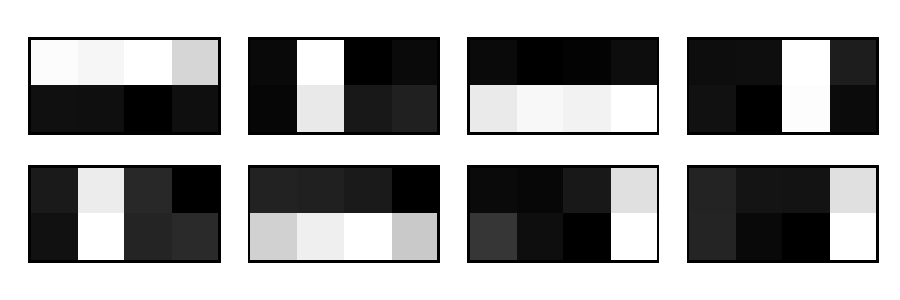
\includegraphics[width=\textwidth]{../code/qcnn/data.pdf}
    \caption{
        Data for the QCNN.
        With a total of 64 training images and 16 for testing, they form balanced dataset of $2\times4$ pixels, with either a vertical or horizontal line encoded as $1$ and $-1$.
        The images are generated with some Gaussian noise.
    }
    \label{fig:qcnn_data}
\end{figure}


First, data is encoded using two repetitions of $Z$ angle encoding, implemented in Qiskit as the \texttt{ZFeatureMap}.
Each of the eight pixels of the image is mapped to a qubit through two repetitions of the Hadamard gate and $Z$-rotations parametrised by the pixel value being applied, in circuit notation:

\begin{equation}
    \begin{quantikz}
        \lstick{$\ket{0}$} & \gate{H} & \gate{R_Z(x_1)} & \gate{H} & \gate{R_Z(x_1)}  \\
        \lstick{$\ket{0}$} & \gate{H} & \gate{R_Z(x_2)} & \gate{H} & \gate{R_Z(x_2)}  \\
        \lstick{\vdots} \\
        \lstick{$\ket{0}$} & \gate{H} & \gate{R_Z(x_n)} & \gate{H} & \gate{R_Z(x_n)}  \\
    \end{quantikz}
\end{equation}



The convolution layers act with pairwise parametrised rotations of neighbouring qubits, also wrapping around, entangling the first and last qubits through various CNOT gates and both parametrised and fixed $Z$ and $Y$ rotations.
Effectively, each consecutive pair of qubits were entangled by
\begin{equation}
    \begin{quantikz}
        &
        \qw
        &
        \targ{}
        &
        \gate{R_Z(\theta_{0})}
        &
        \ctrl{1}
        &
        \qw
        &
        \targ{}
        &
        \gate{R_Z(\pi/2)}
        &
        \qw
        \\
        &
        \gate{R_Z(-\pi/2)}
        &
        \ctrl{-1}
        &
        \gate{R_Y(\theta_{1})}
        &
        \targ{}
        &
        \gate{R_Y(\theta_{3})}
        &
        \ctrl{-1}
        &
        \qw
        &
        \qw
    \end{quantikz}
\end{equation}
giving $3n$ parameters for each convolution layer of $n$ qubits.


Thereafter, pooling layers halve the active qubit counts by parametrised rotations and CNOT gates.
This is done by acting on the first and fifth, second and sixth et cetera with the following circuit:
\begin{equation}
    \begin{quantikz}
        &
        \qw
        &
        \targ{}
        &
        \gate{R_Z(\theta_{0})}
        &
        \ctrl{1}
        &
        \qw
        &
        \qw
        \\
        &
        \gate{R_Z(-\pi/2)}
        &
        \ctrl{-1}
        &
        \gate{R_Y(\theta_{1})}
        &
        \targ{}
        &
        \gate{R_Y(\theta_{3})}
        &
        \qw
    \end{quantikz}
\end{equation}
giving $3n/2$ parameters for each pooling layer of $n$ qubits.

For the final layer, the sole remaining qubit is measured, and the result is interpreted as the prediction.
In total, the circuit appears as

\begin{center}
    \begin{quantikz}
        \lstick[wires=8]{$\ket{0}^{\otimes 8}$} &
        \gate[wires=8, disable auto height]{{\rotatebox{90}{\texttt{ZFeatureMap}$(\bm{x})$}}} &
        \gate[wires=8, disable auto height]{{\rotatebox{90}{\text{Convolution}}}} &
        \gate[wires=8, disable auto height]{{\rotatebox{90}{\text{Pooling}}}} & \qw{}& \qw{}& \qw{}& \qw{} & \qw{}
        \\
        & \qw{}& \qw{}& \qw{}& \qw{}& \qw{}& \qw{}& \qw{}& \qw{}\\
        & \qw{}& \qw{}& \qw{}& \qw{}& \qw{}& \qw{}& \qw{}& \qw{}\\
        & \qw{}& \qw{}& \qw{}& \qw{}& \qw{}& \qw{}& \qw{}& \qw{}\\
        & & & &
        \gate[wires=4, disable auto height]{{\rotatebox{90}{\text{Convolution}}}} &
        \gate[wires=4, disable auto height]{{\rotatebox{90}{\text{Pooling}}}} & \qw{} & \qw{} & \qw{}
        \\
        & \qw{}& \qw{}& \qw{}& \qw{}& \qw{}& \qw{}& \qw{}& \qw{}\\
        & & & & & &
        \gate[wires=2, disable auto height]{{\rotatebox{90}{\text{Conv.}}}} &
        \gate[wires=2, disable auto height]{{\rotatebox{90}{\text{Pooling}}}} & \qw{}

        \\
        & & & & & & & & \meter{} \\
    \end{quantikz}
\end{center}
with a total of 63 parameters.


As in Qiskit's guide, training was done using the COBYLA optimiser\footnote{Constrained Optimisation BY Linear Approximation.} which does not use gradients.
Why this optimiser was chosen is not clear, but testing shows that simulations using gradient based methods such as Adam or simple gradient descent is significantly slower.
The accuracies and loss (mean square error) during training is shown in \cref{fig:qcnn_training}.
Like in \cref{sec:qnn-vs-nn}, noise is modelled after the IBM Montreal hardware.
The networks were trained for 1000 epochs, and while neither reached full accuracy, the losses shrunk, indicating at least increased certainty in the predictions.
Interestingly, the noisy simulation appears to yield better predictions, despite suffering from higher losses during training.
It seems that the noiseless QCNN is overfitting to the training data, while the noisy QCNN generalises better.


\begin{figure}
    \centering
    \begin{subfigure}{0.49\textwidth}
        \centering
        \begin{tikzpicture}
            \begin{axis}[
                    width=\textwidth,
                    height=\textwidth,
                    xlabel={Iteration},
                    ylabel={Loss (MSE)},
                    % legend pos=north west,
                    % legend style={at={(0.5,1.03)},anchor=north},
                    grid=major,
                    xtick distance=200,
                ]
                \addplot[mark=none, color=red] table[x=iteration, y=loss, col sep=comma] {../code/qcnn/noisy.csv};
                \addplot[mark=none, color=blue] table[x=iteration, y=loss, col sep=comma] {../code/qcnn/exact.csv};
                \legend{
                    Noisy QCNN,
                    Exact QCNN,
                }
            \end{axis}
        \end{tikzpicture}
        \caption{}
        \label{fig:qcnn_loss}
    \end{subfigure}
    \begin{subfigure}{0.49\textwidth}
        \centering
        \begin{tikzpicture}
            \begin{axis}[
                    width=\textwidth,
                    height=\textwidth,
                    xlabel={Iteration},
                    ylabel={Accuracy},
                    % legend pos=north west,
                    % legend style={at={(0.5,1.03)},anchor=north},
                    grid=major,
                    legend pos=south east,
                    xtick distance=200,
                ]
                % \addplot[mark=none, color=red] table[x=iteration, y=training_acc, col sep=comma] {../code/qcnn/noisy.csv};
                % \addplot[mark=none, color=red, dashed] table[x=iteration, y=test_acc, col sep=comma] {../code/qcnn/noisy.csv};
                % \addplot[mark=none, color=blue] table[x=iteration, y=training_acc, col sep=comma] {../code/qcnn/exact.csv};
                % \addplot[mark=none, color=blue, dashed] table[x=iteration, y=test_acc, col sep=comma] {../code/qcnn/exact.csv};
                \addplot[mark=none, color=red] table[x=iteration, y=train_mean_noisy, col sep=comma] {../code/qcnn/mean_accs.csv};
                \addplot[mark=none, color=red, dashed] table[x=iteration, y=test_mean_noisy, col sep=comma] {../code/qcnn/mean_accs.csv};
                \addplot[mark=none, color=blue] table[x=iteration, y=train_mean_exact, col sep=comma] {../code/qcnn/mean_accs.csv};
                \addplot[mark=none, color=blue, dashed] table[x=iteration, y=test_mean_exact, col sep=comma] {../code/qcnn/mean_accs.csv};
                \legend{
                    Noisy training,
                    Noisy test,
                    Exact training,
                    Exact test,
                }
            \end{axis}
        \end{tikzpicture}
        \caption{}
        \label{fig:qcnn_acc}
    \end{subfigure}
    \caption{
        Training of the QCNN.
        The red curves are for the noisy model (modelled after IBM's Montreal hardware), while the blue curves are for the exact model.
        The dashed curves are for the test set.
        (a) loss (mean square error) during training.
        (b) accuracy on the training and test sets (running mean with a 100 iteration window).
    }
    \label{fig:qcnn_training}
\end{figure}


\subsection{QCNN with intermediate measurements}
A more complex QCNN structure was described by \textcite{pesah2021}, where the pooling modules measure a qubit and use the result to control a unitary gate on its neighbour.
The use of mid-circuit measurements complicates the circuit and its implementation, but allows for a non-linear and potentially more powerful model.

Following the description in \cite{pesah2021}, a QCNN was implemented with structure as shown in \cref{fig:qcnnm}.
First, the data was encoded using angle encoding in the $X$ direction.
The convolutional layers consisted of pairwise $W$ gates, a mix of parametrised rotations and CNOTs, with total of 15 parameters per gate.
The pooling layers consisted of a measurement and a conditional single-qubit unitary gate.
Without any particular recommendation in the original paper, a simple $X$-gate was used.
Like in \cref{sec:qcnn}, the network used 8 qubits to handle the 8-dimensional data.
Three convolutional and pooling layers were used, reducing the data from 8 to 2 dimensions
Lastly, a final general two-qubit ansatz was used, and a single qubit was measured and interpreted as a prediction.
This was a simple parametrised entangler, similar to the \texttt{RealAmplitudes} in \cref{sec:qnn-vs-nn}, but with $X$ rotations.
In total, the network had 154 parameters.

\begin{figure}
    \centering
    \begin{quantikz}
        % \lstick[wires=4]{$\ket{\psi(\bm{x})}$}
        &
        \qw
        \gategroup[
            wires=4,
            steps=2,
            style={dashed, rounded corners, inner sep=2pt},
            label style={label position=below, anchor=north, yshift=-0.2cm},
        ]{Convolution}
        &
        \gate[wires=2]{W}
        &
        \qw
        &
        \meter{}
        \gategroup[
            wires=4,
            steps=2,
            style={dashed, rounded corners, inner sep=2pt},
            label style={label position=below, anchor=north, yshift=-0.2cm},
        ]{Pooling}
        &
        \cwbend{1}
        \\
        &
        \gate[wires=2]{W}
        &
        \qw
        &
        \qw
        &
        \qw
        &
        \gate{X}
        &
        \qw
        \\
        &
        \qw
        &
        \gate[wires=2]{W}
        &
        \qw
        &
        \qw
        &
        \gate{X}
        &
        \qw
        \\
        &
        \qw
        &
        \qw
        &
        \qw
        &
        \meter{}
        &
        \cwbend{-1}
    \end{quantikz}
    \caption{
        QCNN convolution and pooling layer structure with intermediate measurements.
        Some encoded data or already pooled data enter the convolution layer where parametrised gates $W$ entangle the qubits.
        The pooling modules measure a qubit and use the result to control a unitary gate on a neighbour (here the $X$ gate).
    }
    \label{fig:qcnnm}
\end{figure}

The QCNN was implemented using the PennyLane framework and trained with the Adam optimiser with a learning rate of 0.01.
With the PennyLane implementation, there were no problems using gradient based optimisation.
This prompted the reimplementation of the former QCNN, which was here also trained with the same Adam optimiser.
The results are shown in \cref{fig:qcnnm_training}.
The training loss was lower than for the QCNN in \cref{sec:qcnn}, despite the fewer iterations, showing expected advantages of using gradient based optimisation.
Furthermore, the new model with intermediate measurements achieves a perfect accuracy on both the training and test sets in only 10 iterations.
Looking at the loss curves, it is clear that the new model converges much faster than the old one.

\begin{figure}
    \centering
    \begin{subfigure}{0.49\textwidth}
        \centering
        \begin{tikzpicture}
            \begin{axis}[
                    width=\textwidth,
                    height=\textwidth,
                    xlabel={Iteration},
                    ylabel={Loss (MSE)},
                    % legend pos=north west,
                    % legend style={at={(0.5,1.03)},anchor=north},
                    grid=major,
                    legend pos=north east,
                ]
                \addplot[mark=none, color=blue] table[x=Iteration, y=Loss, col sep=comma] {../code/qcnn_pennylane/results_intermediate.csv};
                \addplot[mark=none, color=red] table[x=Iteration, y=Loss, col sep=comma] {../code/qcnn_pennylane/results_simple.csv};
                % \legend{
                %     New,
                %     Old,
                % }
            \end{axis}
        \end{tikzpicture}
        \caption{}
        \label{fig:qcnnm_loss}
    \end{subfigure}
    \begin{subfigure}{0.49\textwidth}
        \centering
        \begin{tikzpicture}
            \begin{axis}[
                    width=\textwidth,
                    height=\textwidth,
                    xlabel={Iteration},
                    ylabel={Accuracy},
                    % legend pos=north west,
                    % legend style={at={(0.5,1.03)},anchor=north},
                    grid=major,
                    legend pos=south east,
                    xmax=50,
                ]
                \addplot[mark=none, color=blue] table[x=Iteration, y=Accuracy, col sep=comma] {../code/qcnn_pennylane/results_intermediate.csv};
                \addplot[mark=none, color=blue, dashed] table[x=Iteration, y=Test accuracy, col sep=comma] {../code/qcnn_pennylane/results_intermediate.csv};
                \addplot[mark=none, color=red] table[x=Iteration, y=Accuracy, col sep=comma] {../code/qcnn_pennylane/results_simple.csv};
                \addplot[mark=none, color=red, dashed] table[x=Iteration, y=Test accuracy, col sep=comma] {../code/qcnn_pennylane/results_simple.csv};
                % \legend{
                %     New training,
                %     New test,
                %     Old training,
                %     Old test,
                % }
            \end{axis}
        \end{tikzpicture}
        \caption{}
        \label{fig:qcnnm_acc}
    \end{subfigure}
    \caption{
        Training of the QCNNs.
        Blue lines refer to the network with intermediate measurements, while the red are for the network without.
        (a) loss (mean square error) during training.
        (b) accuracy on the training and test sets.
        Solid lines are for the training set, dashed lines for the test set.
        (Note the different ranges of the $x$-axes.)
    }
    \label{fig:qcnnm_training}
\end{figure}
